\section*{Assignment 4}
The task was to bruteforce a 4 digit pin. OOO wow

\emph{Aufgabe: }We had an FPGA configured by the tutors. We should enter it, without any Knowledge what it does.

\subsubsection*{An easy solution}
See figure \ref{fig:as4-schematic-1} (p.~\pageref{fig:as4-schematic-1}).

Bruteforcing the PIN this way took about 30 seconds.

\begin{figure}[tb]
    \begin{center}
        \usetikzlibrary{arrows.meta}
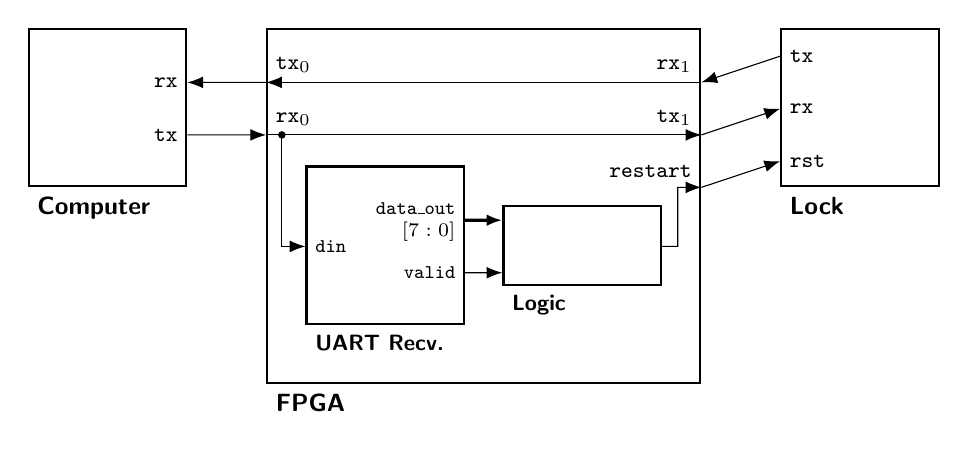
\begin{tikzpicture}
	\tikzstyle{comp} = [
		rectangle, draw=black, thick
	]
	\tikzstyle{component} = [
		comp, minimum width=5.5cm, minimum height=4.5cm
	]
\tikzstyle{component_small} = [
		comp, minimum width=2cm, minimum height=2cm
	]
	\tikzstyle{caption} = [
		below right
	]
	\tikzstyle{conn} = [
		-{Latex[length=2mm]}
	]
	
	% FPGA
	\node (FPGA) [component] at (0,0) {}
		% Caption
		node [caption] at (FPGA.south west) { \small{\textsf{\textbf{FPGA}}} }
		% In/-outputs links
		coordinate [yshift=2.5cm+0.666cm, label={ above right : \footnotesize{$\texttt{rx}_0$} }] (FPGA_rx0) at (FPGA.south west) % unten
		coordinate [yshift=2.5cm+1.333cm, label={ above right : \footnotesize{$\texttt{tx}_0$} }] (FPGA_tx0) at (FPGA.south west) % oben
		% In/outputs  rechts
		coordinate [yshift=2.5cm,                    label={ above left : \footnotesize{$\texttt{restart}$} }] (FPGA_restart) at (FPGA.south east) % unten
		coordinate [yshift=2.5cm+0.666cm, label={ above left : \footnotesize{$\texttt{tx}_1$} }]      (FPGA_tx1)        at (FPGA.south east) % mitte
		coordinate [yshift=2.5cm+1.333cm, label={ above left : \footnotesize{$\texttt{rx}_1$} }]      (FPGA_rx1)        at (FPGA.south east)  % oben
	;

	% Receiver
	\node (Receiver) at (FPGA.south west) [component_small, above right, shift={(0.5, 0.75)}] {}
		% Caption
		node [caption] at (Receiver.south west) { \textsf{\footnotesize{\textbf{UART Recv.}}} }
		% Input rechts
		coordinate [yshift=1cm, label={ right : \scriptsize{\texttt{din}} }] (Receiver_din) at (Receiver.south west)
		% Outpus rechts
		coordinate [yshift=0.666cm,                 label={ left : \scriptsize{\texttt{valid}} }]           (Receiver_valid)           at (Receiver.south east) % unten
		coordinate [yshift=1.333cm+0.15cm, label={ left : \scriptsize{\texttt{data\_out}} }] (Receiver_data_out)    at (Receiver.south east) % oben
		coordinate [yshift=1.333cm-0.15cm,  label={ left : \scriptsize{$[7:0]$} }]                     (Receiver_data_out2) at (Receiver.south east) % mitte
	;

	% Logic
	\node (Logic) at (FPGA.south east) [comp, minimum height=1cm, minimum width=2cm, above left, shift={(-0.5, 1.25)}] {}
		node [caption] at (Logic.south west) { \textsf{\footnotesize{\textbf{Logic}}} }
		% Inputs rechts
		coordinate [yshift=0.166cm] (Logic_in0) at (Logic.south west) % unten
		coordinate [yshift=0.833cm] (Logic_in1) at (Logic.south west) % oben
		% Output link
		coordinate [yshift=0.5cm] (Logic_out) at (Logic.south east)
	;

	% Computer
	\node (Computer) [component_small, below left, xshift=-1cm] at (FPGA.north west) {}
		% Caption
		node [caption] at (Computer.south west) { \small{\textsf{\textbf{Computer}}} }
		% In/outputs rechts
		coordinate [yshift=0.666cm, label={ left:\footnotesize{\texttt{tx}} }] (Computer_tx) at (Computer.south east) % unten
		coordinate [yshift=1.333cm, label={ left:\footnotesize{\texttt{rx}} }] (Computer_rx) at (Computer.south east) % oben
	;

	% Lock
	\node (Lock) [component_small, below right, xshift=1cm] at (FPGA.north east) {}
		% Caption
		node [caption] at (Lock.south west) { \small{\textsf{\textbf{Lock}}} }
		% In/outputs rechts
		coordinate [yshift=0.333cm, label={ right:\footnotesize{\texttt{rst}} }] (Lock_rst) at (Lock.south west) % unten
		coordinate [yshift=0.999cm, label={ right:\footnotesize{\texttt{rx}} }]   (Lock_rx)   at (Lock.south west) % mitte
		coordinate [yshift=1.666cm, label={ right:\footnotesize{\texttt{tx}} }]   (Lock_tx)   at (Lock.south west) % oben
	;

	% Computer -> FPGA
	\draw[conn] (Computer_tx) -- (FPGA_rx0);
	\draw[conn] (FPGA_tx1) -- (Lock_rx);
	\draw[conn] (FPGA_restart) -- (Lock_rst);
	
	% FPGA -> Computer
	\draw[conn]  (Lock_tx) -- (FPGA_rx1) ;
	\draw[conn]  (FPGA_tx0) -- (Computer_rx);
	
	% FPGA internal
	\draw[conn] (FPGA_rx0) -- (FPGA_tx1);
	\draw[conn]  (FPGA_rx1) -- (FPGA_tx0);
	\draw[fill=black] (FPGA_rx0) +(0.2,0) circle (0.4mm);
	\draw[conn] (FPGA_rx0) +(0.2,0) |- (Receiver_din);
	\draw[conn] (Receiver_valid) -- (Logic_in0);
	\draw[conn, very thick] (Receiver_data_out) +(0, -0.15) -- (Logic_in1);
	\coordinate [xshift=0.2cm] (h1) at (Logic_out);
	\coordinate [yshift=0.75cm] (h2) at (h1);
	\draw[conn] (Logic_out) -- (h1) -- (h2) -- (FPGA_restart);

\end{tikzpicture}
        \caption{In this setup, all possible PINs are computed on the computer and transmitted to the device. The FPGA just relays the communication and understands the computers' output bitstream to reset the mircrocontroller upon receiving a special command.}
        \label{fig:as4-schematic-1}
        \vspace{1em}\hrule
    \end{center}
\end{figure}

\emph{Bearbeitung und Lösung: }Wenn die Von den Tutoren Programmierte FPGA (FPGA-PIN) über den Throughput an den Computer anschloss und die resettaste des FPGA-PIN betätigte, Würde man auf dem Cmputerbildschirm zur eingabe eines PINs aufgefordert. Nach der eingabe von Vier Ziffern zeigte der Computer an das der Pin falsch sei \emph{"Incorrect Pin"}. erst nache inigen Sekunden war es wieder möglich erneut einen Pin einzugeben. 
Der Lösungsansatz war trozdem eine Implementierung eines Brutforce algotythmus. Um die Wartezeit nach einer Falscheingabe zu umgehen, wurde jedoch der Reset Pin des FPGA-Pin angeprochen um die FPGA zu resetten und so sofort einen neuen Pin eingeben zu können. 
Um den Brutforce algorythmus auf dem FPGA zu realisieren, Bauten wir eine State Mashine mit 4 Zuständen, einem UART-Transmitter und einem UART-Reciver.

\subsubsection*{The fast way}
See figure \ref{fig:as4-schematic-2} (p.~\pageref{fig:as4-schematic-2}).

Compared to the first approach, this solution is magnitues faster requiring only about 3 seconds to obtain the PIN.

\begin{figure}[tb]
    \begin{center}
        \usetikzlibrary{arrows.meta}
\usetikzlibrary{calc,intersections,through,backgrounds}
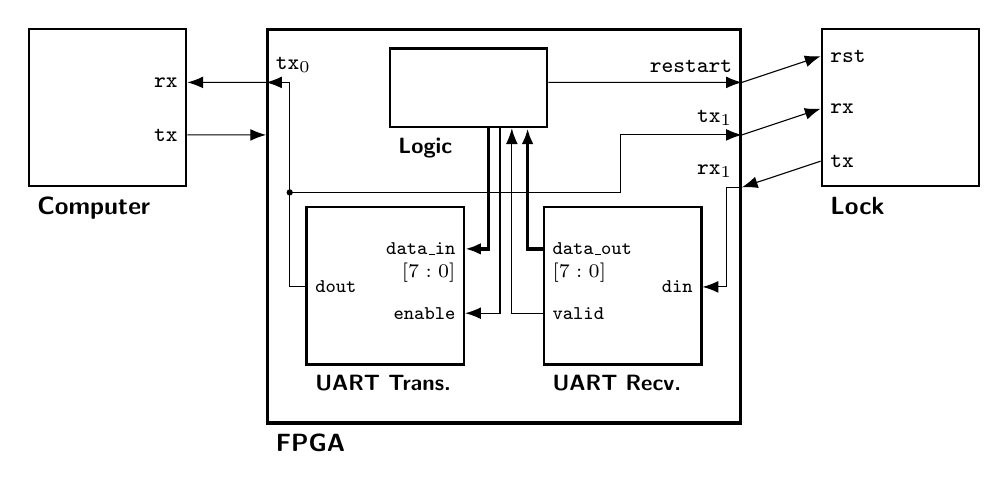
\begin{tikzpicture}
% 	\tikzset{
% 	  every node/.style={scale=1.1}
% 	}	
	\tikzset{comp/.style={
		rectangle, draw=black, thick
	}}	
	\tikzset{component/.style={
		comp, minimum width=6cm, minimum height=5cm, very thick
	}}
	\tikzset{component_small/.style={
		comp, minimum width=2cm, minimum height=2cm, thick
	}}
	\tikzset{caption/.style={
		below right
	}}
	\tikzset{conn/.style={
		-{Latex[length=2mm]}
	}}
	
	% FPGA
	\node (FPGA) [component] at (0,0) {}
		% Caption
		node [caption] at (FPGA.south west) { \small{\textsf{\textbf{FPGA}}} }
		
		% In/-outputs links
		coordinate [yshift=3cm+0.4pt+0.666cm, label={ above right : \footnotesize{} }]                           (FPGA_rx0) at (FPGA.south west) % unten
		coordinate [yshift=3cm+0.4pt+1.333cm, label={ above right : \footnotesize{$\texttt{tx}_0$} }] (FPGA_tx0) at (FPGA.south west) % oben

		% In/outputs  rechts
		coordinate [yshift=3cm+0.4pt,                    label={ above left : \footnotesize{$\texttt{rx}_1$} }]      (FPGA_rx1)       at (FPGA.south east)  % unten
		coordinate [yshift=3cm+0.4pt+0.666cm, label={ above left : \footnotesize{$\texttt{tx}_1$} }]      (FPGA_tx1)       at (FPGA.south east) % mitte
		coordinate [yshift=3cm+0.4pt+1.333cm, label={ above left : \footnotesize{$\texttt{restart}$} }] (FPGA_restart) at (FPGA.south east) % oben
	;

	% Logic
	\node (Logic) at (FPGA.north) [comp, minimum height=1cm, minimum width=2cm, below, shift={(-0.45cm, -0.25cm)}] {}
		node [caption] at (Logic.south west) { \textsf{\footnotesize{\textbf{Logic}}} }
	;

	% Receiver
	\node (Receiver) at (FPGA.south east) [component_small, above left, shift={(-0.5, 0.75)}] {}
		% Caption
		node [caption] at (Receiver.south west) { \textsf{\footnotesize{\textbf{UART Recv.}}} }

		% Input rechts
		coordinate [yshift=1cm, label={ left : \scriptsize{\texttt{din}} }] (Receiver_din) at (Receiver.south east)

		% Outpus links
		coordinate [yshift=0.666cm,                 label={ right : \scriptsize{\texttt{valid}} }]           (Receiver_valid)           at (Receiver.south west) % unten
		coordinate [yshift=1.333cm+0.15cm, label={ right : \scriptsize{\texttt{data\_out}} }] (Receiver_data_out)    at (Receiver.south west) % oben
		coordinate [yshift=1.333cm-0.15cm,  label={ right : \scriptsize{$[7:0]$} }]                     (Receiver_data_out2) at (Receiver.south west) % mitte
	;

	% Transmitter
	\node (Transmitter) at (FPGA.south west) [component_small, above right, shift={(0.5, 0.75)}] {}
		node [caption] at (Transmitter.south west) { \textsf{\footnotesize{\textbf{UART Trans.}}} }

		% Output links
		coordinate [yshift=1cm, label={ right: \scriptsize{\textsf{\texttt{dout}}} }] (Transmitter_dout) at (Transmitter.south west) % unten

		% Inputs links
		coordinate [yshift=0.666cm,                 label={ left : \scriptsize{\texttt{enable}} }]    (Transmitter_enable)   at (Transmitter.south east) % unten
		coordinate [yshift=1.333cm-0.15cm,  label={ left : \scriptsize{$[7:0]$} }]                  (Transmitter_data_in2)at (Transmitter.south east) % mitte
		coordinate [yshift=1.333cm+0.15cm, label={ left : \scriptsize{\texttt{data\_in}} }] (Transmitter_data_in)  at (Transmitter.south east) % oben	
	;

	% Computer
	\node (Computer) [component_small, below left, xshift=-1cm] at (FPGA.north west) {}
		% Caption
		node [caption] at (Computer.south west) { \small{\textsf{\textbf{Computer}}} }

		% In/outputs rechts
		coordinate [yshift=0.666cm, label={ left:\footnotesize{\texttt{tx}} }] (Computer_tx) at (Computer.south east) % unten
		coordinate [yshift=1.333cm, label={ left:\footnotesize{\texttt{rx}} }] (Computer_rx) at (Computer.south east) % oben
	;

	% Lock
	\node (Lock) [component_small, below right, xshift=1cm] at (FPGA.north east) {}
		% Caption
		node [caption] at (Lock.south west) { \small{\textsf{\textbf{Lock}}} }

		% In/outputs rechts
		coordinate [yshift=0.333cm, label={ right:\footnotesize{\texttt{tx}} }]   (Lock_tx)   at (Lock.south west) % unten
		coordinate [yshift=0.999cm, label={ right:\footnotesize{\texttt{rx}} }]   (Lock_rx)   at (Lock.south west) % mitte
		coordinate [yshift=1.666cm, label={ right:\footnotesize{\texttt{rst}} }] (Lock_rst)  at (Lock.south west) % oben
	;

	% Computer <-> FPGA
	\draw[conn]  (FPGA_tx0) -- (Computer_rx);
	\draw[conn] (Computer_tx) -- (FPGA_rx0);

	% FPGA <-> Lock
	\draw[conn] (FPGA_restart) -- (Lock_rst);
	\draw[conn] (FPGA_tx1) -- (Lock_rx);
	\draw[conn] (Lock_tx) -- (FPGA_rx1) ;
	
	% FPGA internal
		\draw[conn] ([yshift=0.583cm] Logic.south east) -- (FPGA_restart);
	
		% Connections to/from Receiver
		\draw[conn] (FPGA_rx1) -- ([xshift=-0.2cm] FPGA_rx1) |- (Receiver_din);
		\draw[conn, very thick] (Receiver_data_out) -| ([xshift=0.75cm] Logic.south); 
		\draw[conn] (Receiver_valid) -| ([xshift=0.55cm] Logic.south);
		
		% Connections to/from Transmitter
		\draw[conn, very thick] ([xshift=0.25cm]Logic.south) |- (Transmitter_data_in);
		\draw[conn] ([xshift=0.4cm] Logic.south) |- (Transmitter_enable);
		\draw[conn, name path=Transmitter_dout--FPGA_tx0] (Transmitter_dout) -- ([xshift=-0.2cm] Transmitter_dout) |- (FPGA_tx0);
		\draw[conn, name path=Transmitter_dout--FPGA_tx1] ([shift={(-0.2cm, 1.2cm)}] Transmitter_dout) -- ([shift={(4cm, 1.2cm)}] Transmitter_dout) |- (FPGA_tx1);

		% Intersection
		\fill[name intersections={of=Transmitter_dout--FPGA_tx0 and Transmitter_dout--FPGA_tx1, total=\t}] (intersection-\t) circle (0.4mm);
\end{tikzpicture}
        \caption{Now the FPGA calculates the 4 digit numbers, sends them to the device and decodes the answer bitstream in order to reset the microcontroller. The computer is passive in this configuration and only needed as output device, so we safely ignore its transmissions.}
        \label{fig:as4-schematic-2}
        \vspace{1em}\hrule
    \end{center}
\end{figure}


\begin{itemize}


\item[START] Ist der erste Zustand der STate mashine, in dem die 4 stellen des Pins sowie einem 5. Übertragszahl auf 0 gesetzt. diese 5 Ziffern werden als 8-Bit gehandhabt. Außerdem werden andere Register initialisiert.

\item[SEND] In diesem Zustand das erste Byte des 4 Stelligen Pins an den UART-Tranmitter übergeben, welcher es direkt an die FPGA-Pin weiterleitet. nun werden alle stellen des Pins um eine stelle verrückt, wobei die vorher erste stelle auf die Hilfvariable übertragen wird. Nun wird der Vorgang wiederholt und die neue erste Stelle des Pins via Transmitter übermittelt. Dieser vorgang findet statt, bis alle zeichen wieder an ihrem orginalen ort sind. 

\item[INC] Hier wird Die nidrigste Stelle des Pins um 1 erhöht. ist diese Stelle bereits 9 muss der übertrag berücksichtigt werden. Außerdem wird der Aktuelle Pin an den Computer Übergeben, um den Vortgang verfolgen zu können.

\item[RECIVE] in diesem Zustand wird auf die Antwort des FPGA-Pin gewartet. Beginnt die Antwort mit einem "I" wie bei Incorrect Pin, wird die Resetfunktion des FPGA-Pin betätigt und die Statmashine begibt sich wieder in den SEND zustand und setzt die Bruteforce Attacke fort.

\end{itemize}


